% Chapter 3

\chapter{Application of a Neural Network to Pixel Clustering} % Chapter title

\label{sec:NN} % For referencing the chapter elsewhere, use \autoref{ch:mathtest}

%----------------------------------------------------------------------------------------

%----------------------------------------------------------------------------------------

\section{Clustering in the Pixel Detector}

Creating tracks from individual hits in the Inner Detector is one of most computationally challenging parts of the reconstruction of ATLAS events. Each event typically contains thousands of hits in the pixel detector alone, which must be combined into one coherent picture of which particles traversed the detector, and how they moved and lost energy as they traveled. A typical particle deposits charge in several pixels per layer, forming a series of clusters which can be connected together to form a track. This track can in turn be used to measure the charge, momentum, and trajectory of the particle, and in many cases, provides ATLAS's most precise measurement of a charged particle. 


\begin{centering}
\begin{figure}[bth]
\myfloatalign
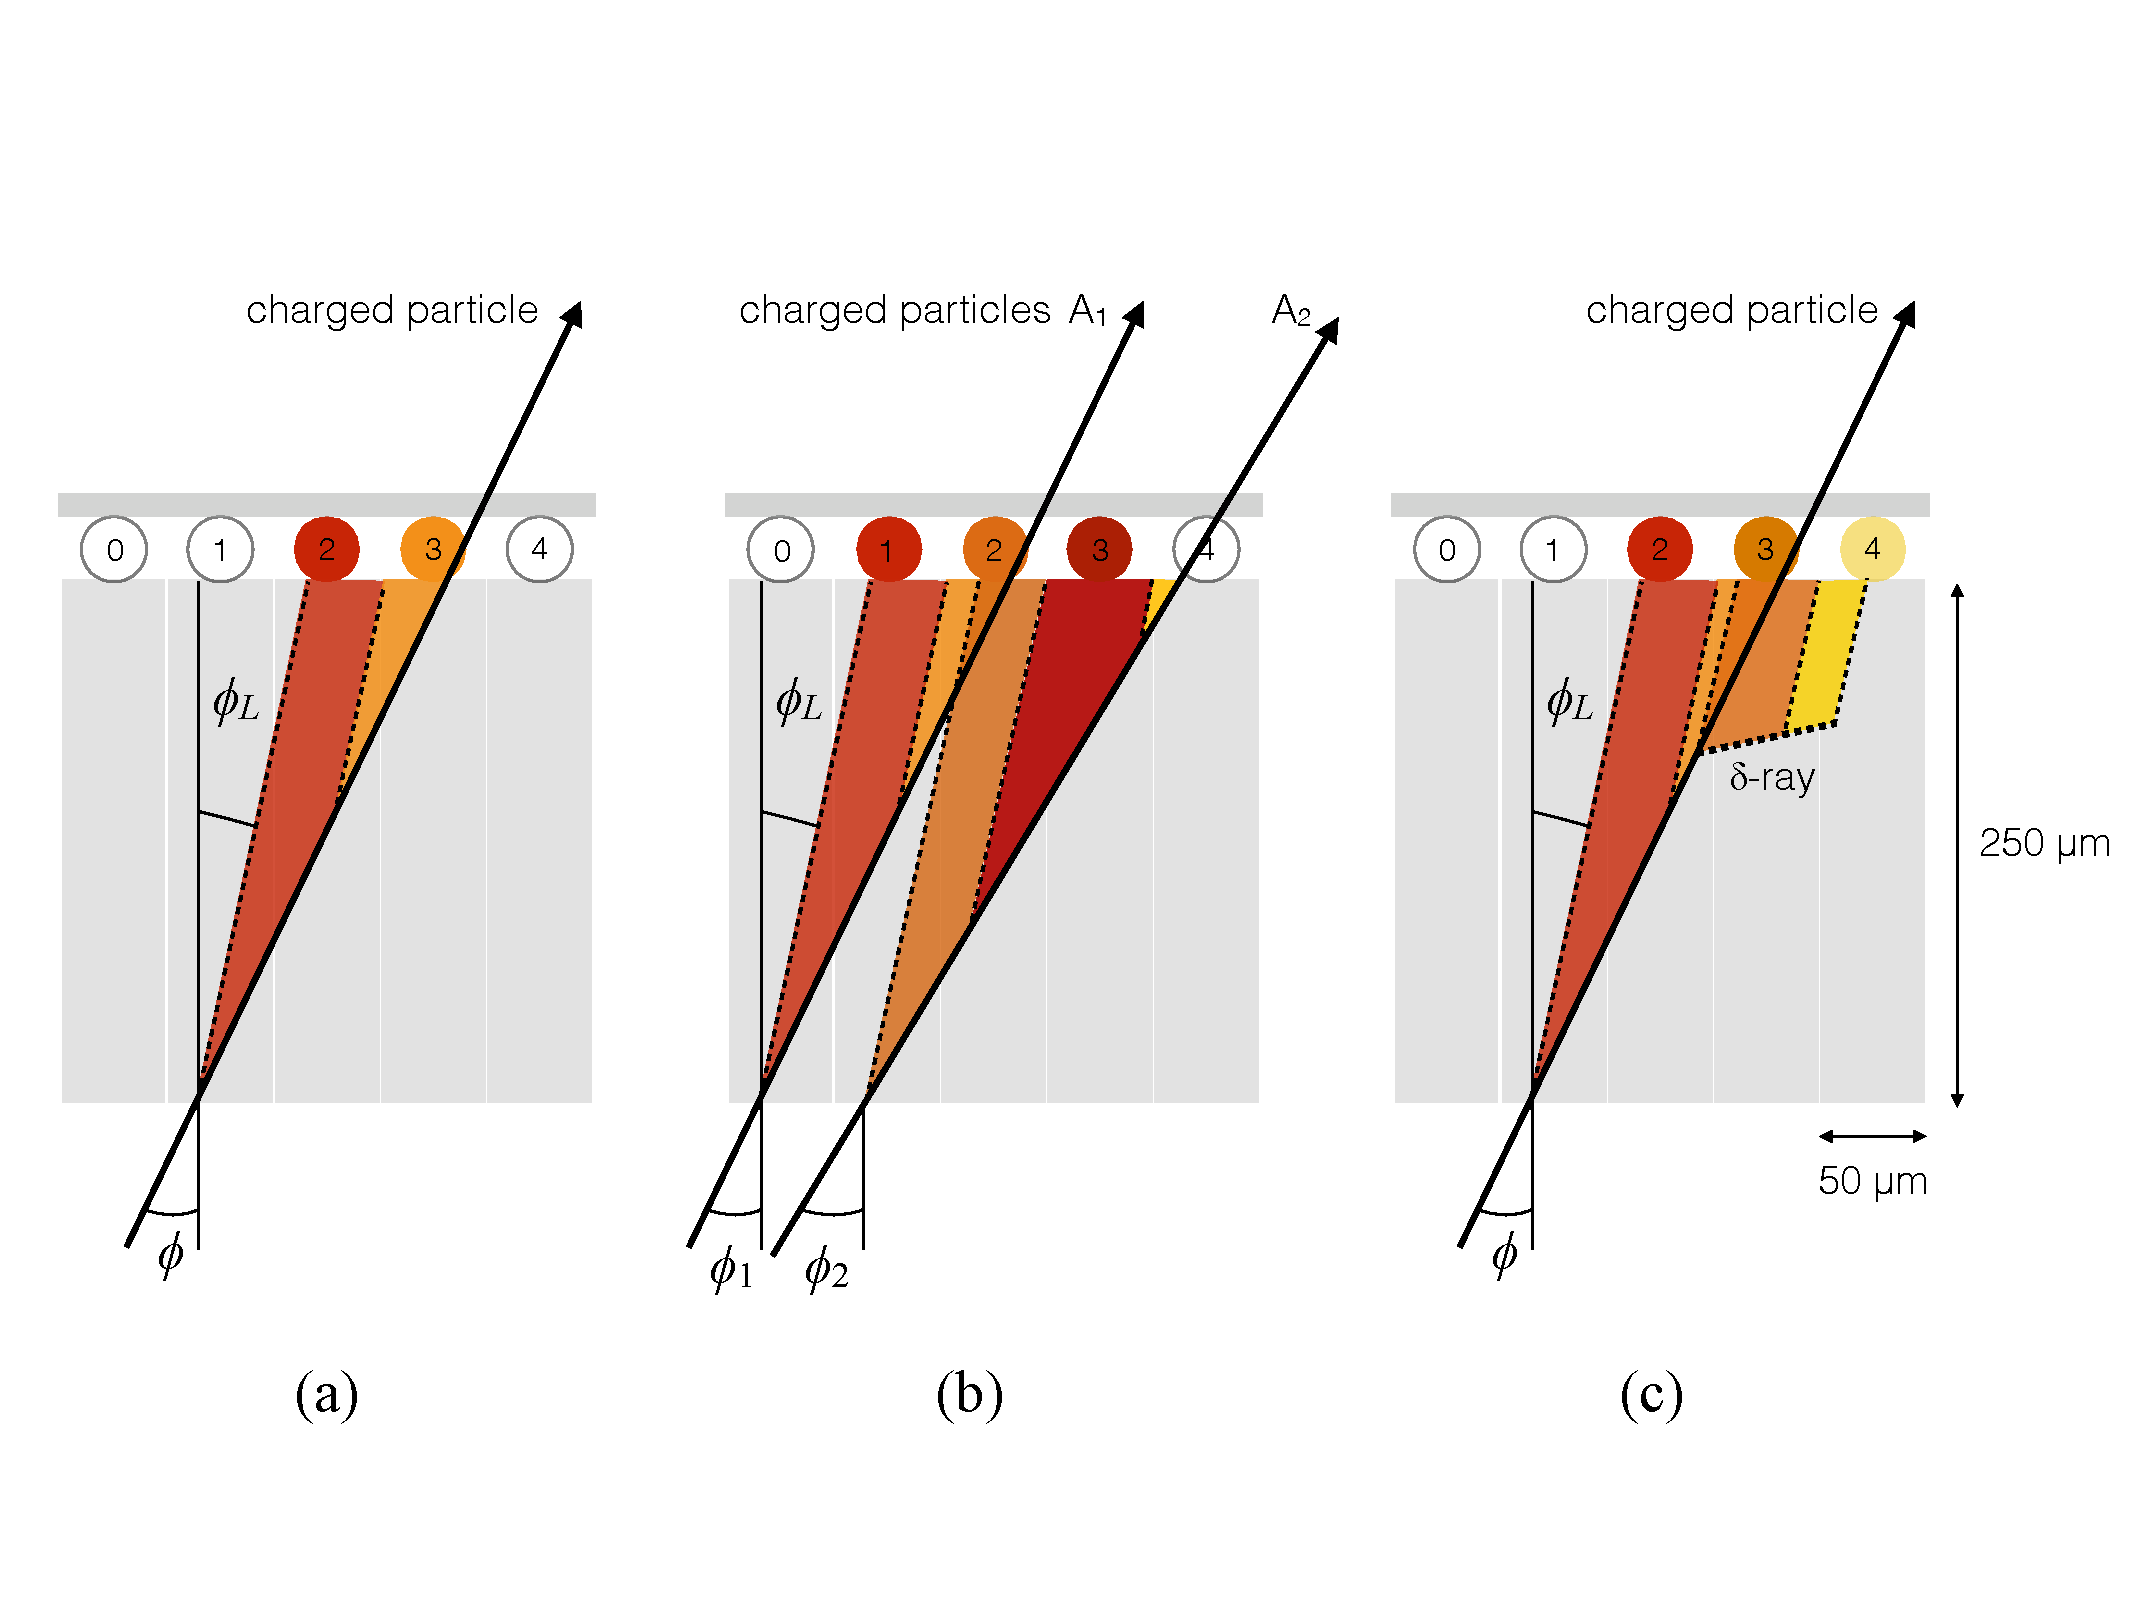
\includegraphics[width=.90\linewidth]{figures/nn/cluster_types.pdf}
\caption{A few possible types of clusters in the Pixel Detector. $(a)$ shows a single particle passing through a layer of the detector, $(b)$ shows two particles passing through the detector, creating a single merged cluster, and $(b)$ shows a single particle emitting a $\delta$-ray as it passes through the detector.}
\label{fig:cluster_types}
\end{figure}
\end{centering}

The process of going from clusters to track is relatively simple in an isolated environment in which one particle travels cleanly through all the layers, but can be complicated by multiple close-by tracks and by a single particle's emission of low energy particles, called $\delta$-rays. In these cases, it can be hard to tell how many particles were involved in creating a cluster, and where exactly each of those particles passed through the layer. A few examples of these cases can be seen in \autoref{fig:cluster_types} . The process of determining this is called Clustering, and it has recently been updated from a charge interpolation method to a method using a \ac{NN}. 

\subsection{Charge Interpolation Method}

A typical cluster contains a few pixel hits spanning in the $x$ and $y$ directions, each with its own measurement of charge deposition, or \ac{ToT}. The extent of the cluster is defined by grouping together any pixels with a shared edge or corner. In the charge interpolation method, also called the \ac{CCA} clustering algorithm, these individual hits are combined to make one estimation of the position a single particle which passed through them, using the following equation: 

\begin{eqnarray}
x_{cluster} = x_{center} + \Delta_x(\phi,N_{row}) \cdot \left[ \Omega_x -\frac{1}{2} \right] \\
\label{eq:analogx}
x_{cluster} = x_{center} + \Delta_x(\phi,N_{row}) \cdot \left[ \Omega_x -\frac{1}{2} \right]
\label{eq:analogy}
\end{eqnarray}

where $\Omega_{x(y)}$ is defined by

\begin{equation}
\Omega_{x(y)} = \frac{q_{last~row(col)}}{q_{first~row(col)} + q_{last~row(col)}}
\end{equation}

and $q$ represents the \ac{ToT} of a given pixel, and $\Delta_{x(y)}$ is a function derived from either data or \ac{MC} and produces an output related to the projected length of the particles track on the pixel sensor and is measured as a function of $\phi$, the incident angle of a particle on the sensor, and $N_{row(col)}$, the number of pixels in the $x$ and $y$ direction. 

In a simple case, such as $(a)$ of \autoref{fig:cluster_types} , this method works quite effectively. However, in cases like $(b)$, it has no ability distinguish two-particle from one-particle clusters, and can only assign a cluster center between the two particles' locations, despite that intermediate pixel having the lowest \ac{ToT}. Furthermore, because this method can't differentiate two-particle clusters, the tracking software can't use that information to preferentially allow multiple tracks to be fit to the cluster. In cases like $(c)$, the $\delta$-ray will bias the measurement of the particle's position in whichever direction it is emitted. 

\subsection{Improving Measurement with Neural Networks}

To address these problems, a series of \acp{NN} were created \cite{PERF-2012-05}. The first determines the number of particles in a given cluster, the second predicts their positions with the cluster, and the third assesses the resolution of the position measurement. 

These \acp{NN} are all trained with: 
\begin{itemize}
\item a $7\times7$ grid of cluster \ac{ToT} information\footnote{Clusters spanning more than seven pixels in either direction are split into multiple clusters.}
\item a seven-element vector containing the $y$-size of the pixels in the grid
\item the layer number of the cluster
\item a variable indicating whether the cluster located in the barrel or endcap
\item $\theta$ and $\phi$ variables projecting the incident angles of the particle on the sensor, assuming it comes from the interaction point
\item the $\eta$ index of the pixel module
\end{itemize}

After the Number \ac{NN} predicts a number of particles associated with the cluster, required to be between 1 and 3, the same inputs are fed to one of three Position \acp{NN} based on the determined number of particles, which then outputs the $x$ and $y$ positions of each of the particles. Then, the same inputs combined with the output of the Position \ac{NN} are fed into one of three Error \acp{NN} (also distinguished by number of particles), which outputs a resolution for each of the position predictions made. An example of the output of this process can be seen in \autoref{fig:merged_cluster}, where the improved position resolution from the ability to identify a multi-particle cluster is evident. The particle location predictions from the \acp{NN} are then handed to the tracking software, which is able to independently consider multiple locations from a given cluster to find the best fit. 

\begin{centering}
\begin{figure}[bth]
\myfloatalign
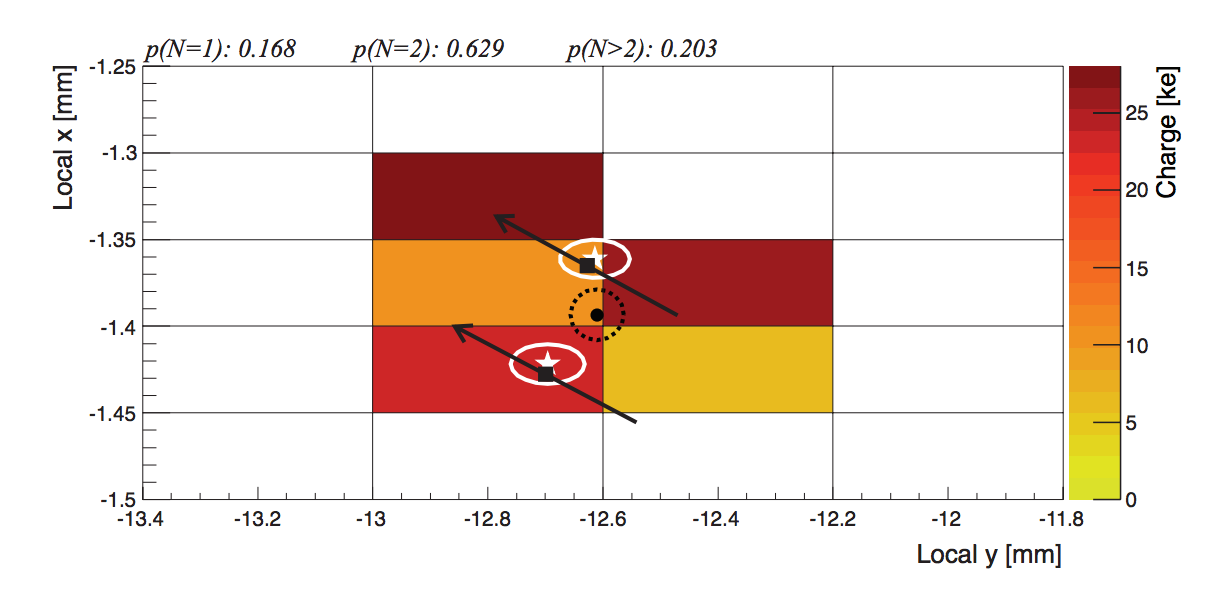
\includegraphics[width=.90\linewidth]{figures/nn/merged_cluster.png}
\caption{One example of a two-particle cluster and its truth information compared with the output of the \acp{NN}. At top, the $p(N=i)$ values give the output of the Number \ac{NN}, the probabilities that the cluster contains 1, 2, and 3 particles. Given the highest probability is for $N=2$, the other \acp{NN} predict the postion and errors of the two particles (in white). The black arrows and squares represent the truth information from the cluster, and the black dot and dotted line show the position measurement for the un-split cluster.}
\label{fig:merged_cluster}
\end{figure}
\end{centering}

\section{Impact of the Neural Network}

The \ac{NN} was first applied to $7 TeV$ data, where it improved position resolution for particles in small and large clusters. \autoref{fig:7tev_res} shows the improvement from the addition of the \ac{NN} in $x$ resolution in different cluster sizes. The improvement from \ac{CCA} clustering is particularly evident in the 4-pixel case, where the double peaked structure of the interpolation method has been completely removed with the \ac{NN}.  

\begin{centering}
\begin{figure}[bth]
\myfloatalign
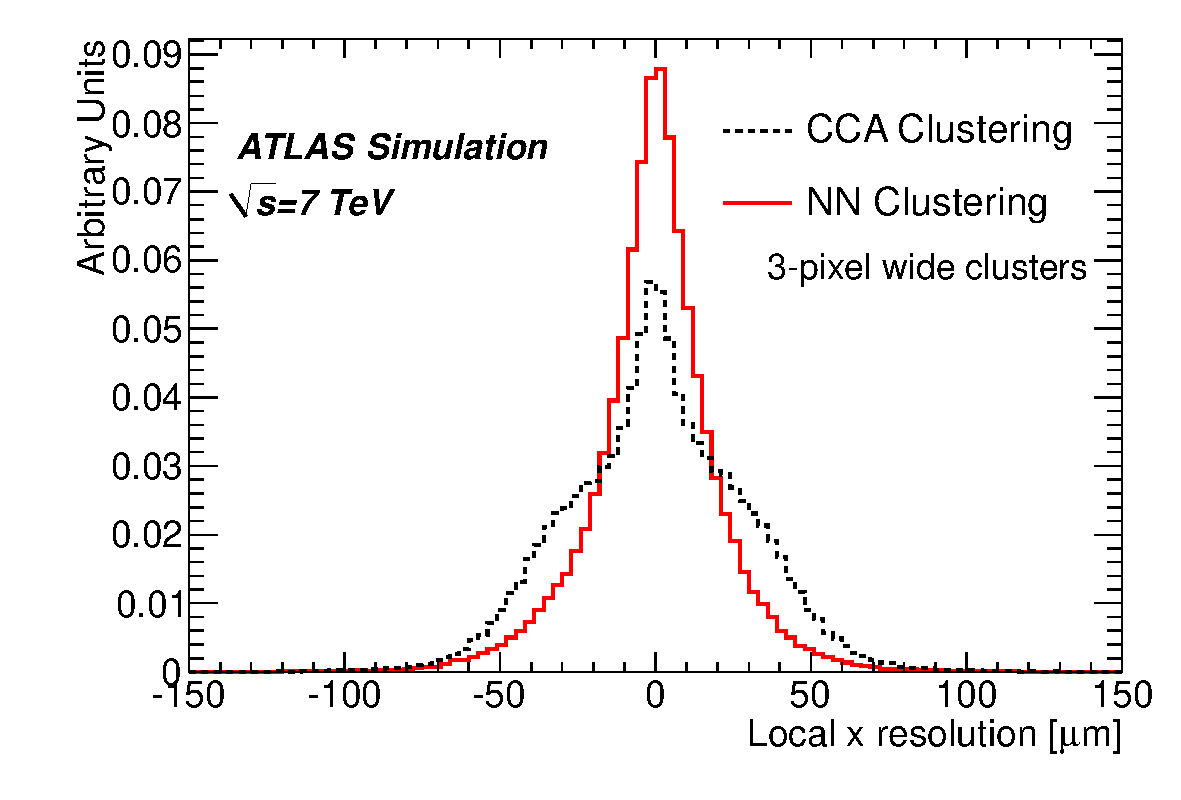
\includegraphics[width=.45\linewidth]{figures/nn/3x_res.pdf}
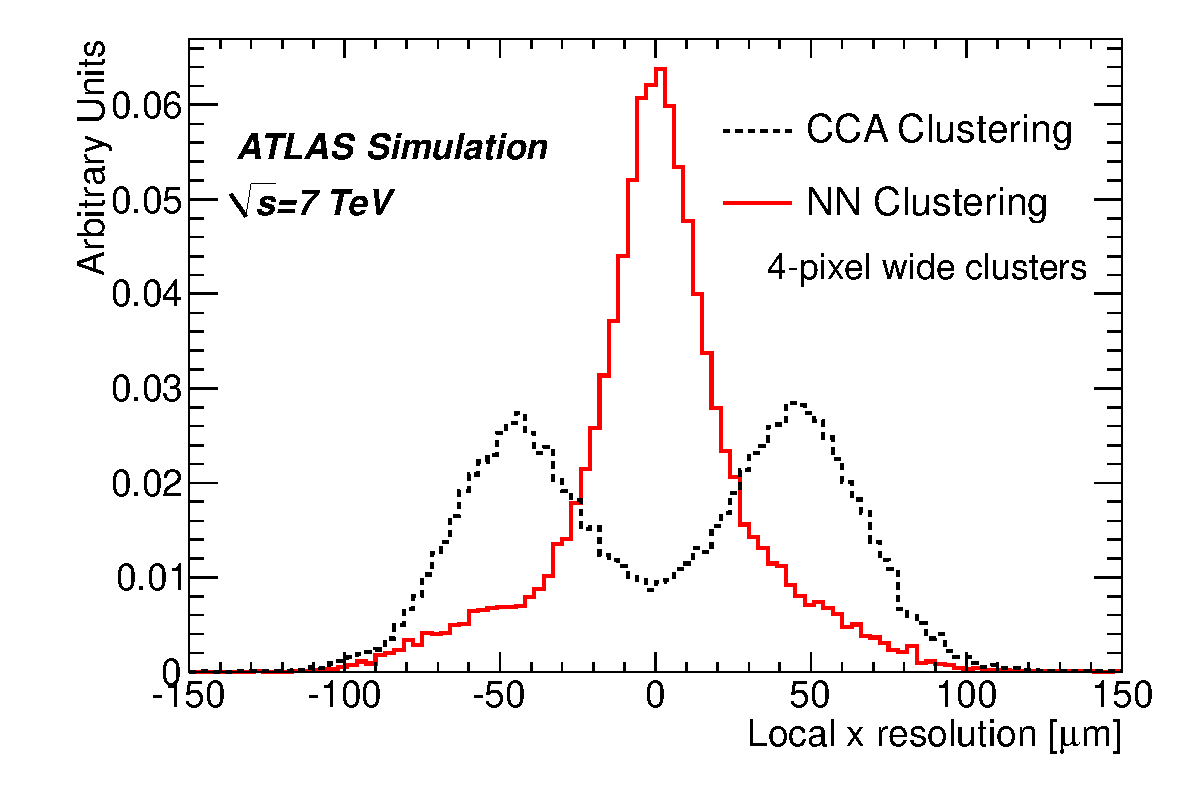
\includegraphics[width=.45\linewidth]{figures/nn/4x_res.pdf}
\caption{$x$ resolutions for clusters with 3 (left) and 4 (right) pixels in the $x$ direction in $7 TeV$ data for \ac{CCA} and \ac{NN} clustering.}
\label{fig:7tev_res}
\end{figure}
\end{centering}

\subsection{The Neural Network in 13 TeV Data}

In Run 2, tracking algorithm is first run on the \ac{CCA} clusters, where it constructs loose tracks that allow shared clusters, clusters to which multiple tracks are fit. The \ac{NN} is then used to identify which clusters are likely to have had multiple particles pass through them, and to identify the positions of those particles. In the case that the cluster is determined to have resulted only from one particle, tracks that share that cluster are penalized. 

Performance in 13 TeV \cite{ATL-PHYS-PUB-2015-044}. 

Robustness \cite{ATL-PHYS-PUB-2015-052}
